\begin{figure}[]
        \center{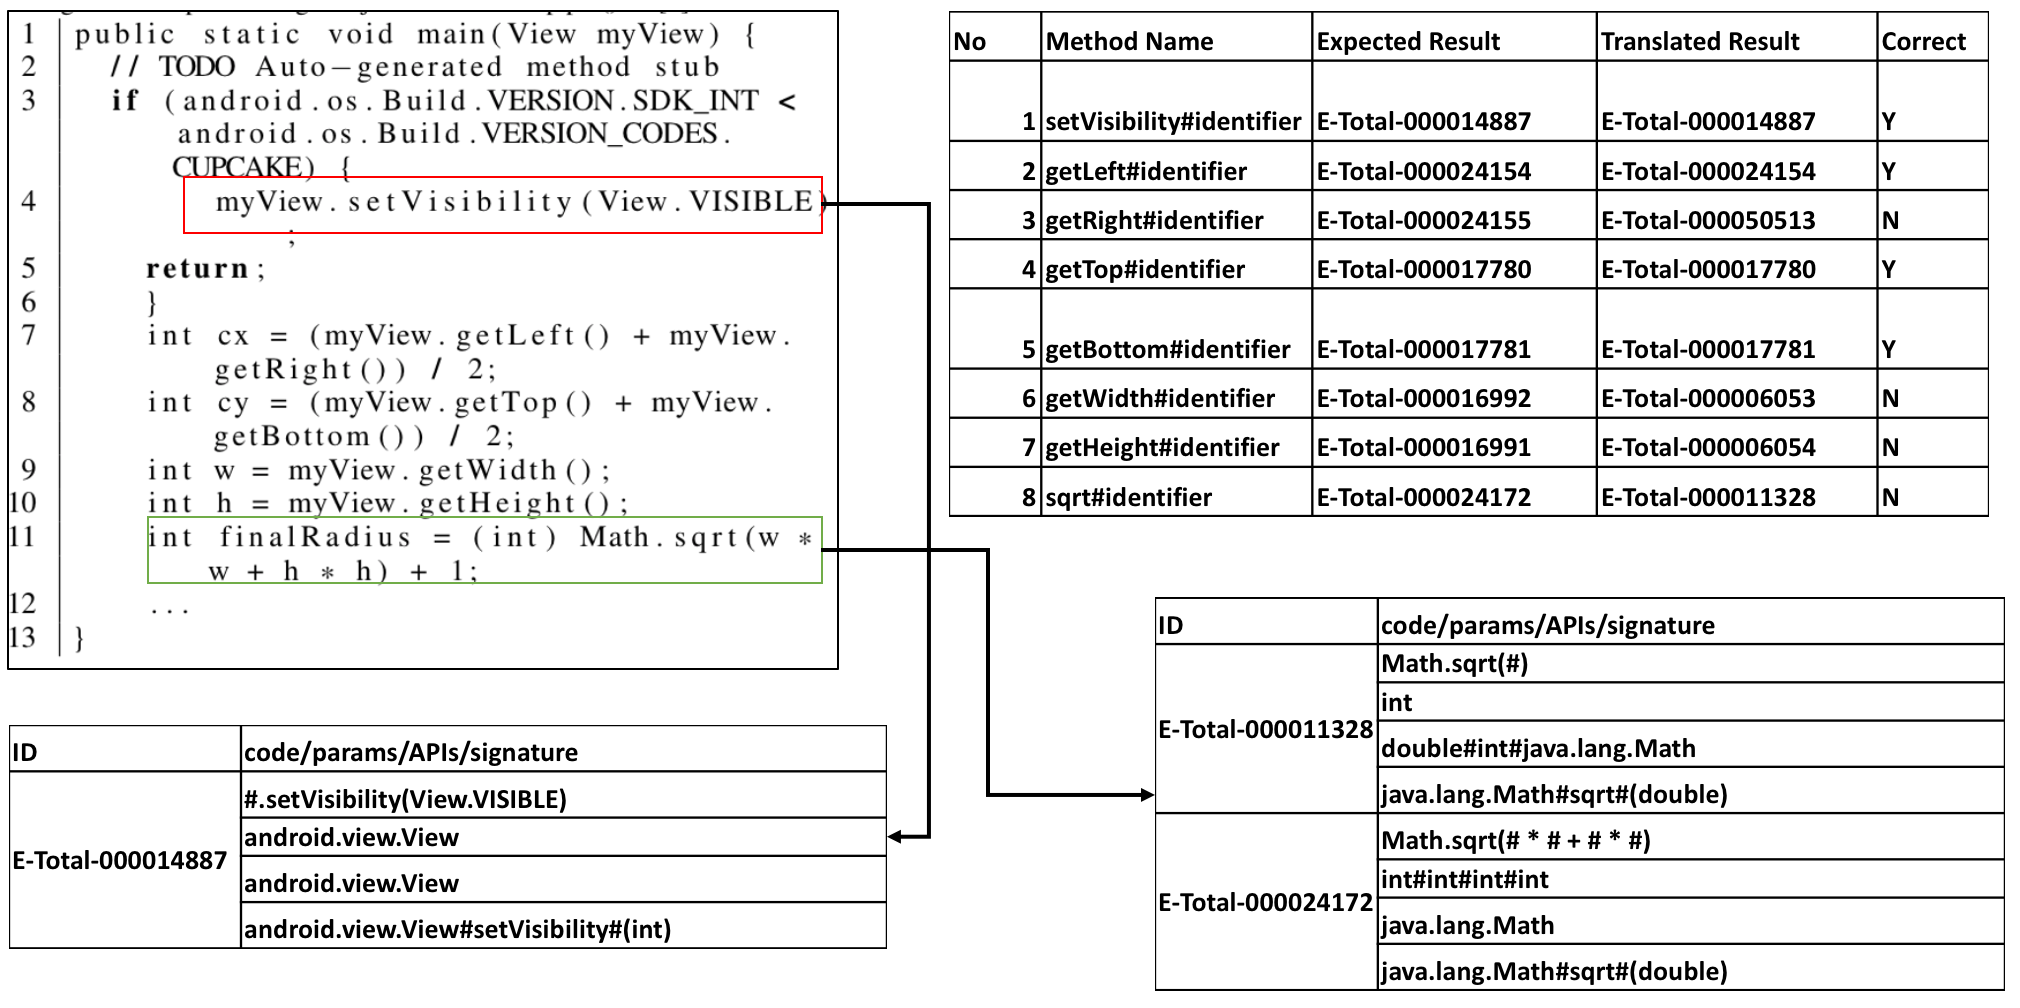
\includegraphics[width=\linewidth]
        {images/android_3.png}}
        \caption{\label{fig:android_example} Example of query in configuration 1 for code snippet in \cite{id:ProgramCreekAndroidExample}}
      \end{figure}

We study the results with configuration 1. An example of the code snippet we collected from Program Creek in the post \cite{id:ProgramCreekAndroidExample} is shown in Figure \ref{fig:android_example}. The output of translation is the list of ASTs represented by their ID. We can see that if a developer writes \texttt{"set visibility"} and give the context since the developer wants to do some calculation relating to the position of the \texttt{View} object, the SMT model will automatically suggest an AST that set visibility to true of the correct receiver. Incorrect translated results often happened if developer inputs about a method name on complicate expression. In this example, if the developer inputs \texttt{"sqrt"}, the translated result is to accept a single integer variable, while the correct result requires four integers as parameters.   